
\let\negmedspace\undefined
\let\negthickspace\undefined
\documentclass[journal,12pt,onecolumn]{IEEEtran}

\usepackage{cite}
\usepackage{amsmath,amssymb,amsfonts,amsthm}
\usepackage{algorithmic}
\usepackage{graphicx}
\graphicspath{{./figs/}}
\usepackage{textcomp}
\usepackage{xcolor}
\usepackage{txfonts}
\usepackage{listings}
\usepackage{enumitem}
\usepackage{mathtools}
\usepackage{gensymb}
\usepackage{comment}
\usepackage{caption}
\usepackage[breaklinks=true]{hyperref}
\usepackage{tkz-euclide}
\usepackage{listings}
\usepackage{gvv}
\usepackage[latin1]{inputenc}
\usepackage{xparse}
\usepackage{color}
\usepackage{array}
\usepackage{longtable}
\usepackage{calc}
\usepackage{multirow}
\usepackage{multicol}
\usepackage{hhline}
\usepackage{ifthen}
\usepackage{lscape}
\usepackage{tabularx}
\usepackage{array}
\usepackage{float}

\begin{document}

\title{8.4.23}
\author{EE25BTECH11020 - Darsh Pankaj Gajare}
{\let\newpage\relax\maketitle}

Question:\\
The curve described parametrically by $x=t^2+t+1$ and $y=t^2-t+1$ represents:

\begin{multicols}{4}
\begin{enumerate}
\item a pair of straight lines
\item an ellipse
\item a parabola
\item a hyperbola
\end{enumerate}
\end{multicols}

\solution
\begin{table}[H]
	\centering
	\caption{}
	\begin{tabular}{|c|c|}
\hline
\textbf{Name} & \textbf{Value} \\ \hline
$\vec{A}$ & $\myvec{2 & 1 \\0 & 3}$ \\ \hline
\end{tabular}

	\label{}
\end{table}

The parametric form can be written as
\begin{align}
\vec{x} &= \vec{a}t^2 + \vec{b}t + \vec{c}.
\end{align}
\begin{align}
	\vec{x}=\myvec{\vec{a}\\\vec{b}}^\top\myvec{t^2\\t}+\vec{c}
\end{align}
\begin{align}
\vec{x}=\myvec{1 & 1\\ 1 & -1}\myvec{t^2\\ t}+\vec{c}
\end{align}

\begin{align}
\myvec{t^2\\ t}=\frac{1}{2}\myvec{1 & 1\\ 1 & -1}
\brak{\vec{x}-\vec{c}}
\end{align}

\begin{align}
\text{Let } \vec{e}_1=\myvec{1\\ 0},\ \vec{e}_2=\myvec{0\\ 1},\ 
\end{align}
\begin{align}
	\vec{M}=\frac{1}{2}\myvec{1 & 1\\ 1 & -1},\ 
\vec{z}=\vec{x}-\vec{c}. 
\end{align}

\begin{align}
	\text{Then } \myvec{t^2\\ t}=\vec{M}\vec{z},\quad
	t^2=\vec{e}_1^\top \vec{M}\vec{z},\quad
	t=\vec{e}_2^\top \vec{M}\vec{z}.
\end{align}

\begin{align}
\text{Eliminate } t:\quad
	\vec{e}_1^\top \vec{M}\vec{z}
=
	\brak{\vec{e}_2^\top \vec{M}\vec{z}}^{2}.
\end{align}

\begin{align}
	\text{Define } \vec{w}=\vec{M}\vec{z}\ \Rightarrow\
\vec{e}_1^\top\vec{w}=\brak{\vec{e}_2^\top\vec{w}}^{2}.
\end{align}

\begin{align}
\text{In matrix form: }\
	\vec{z}^\top \vec{M}^\top \vec{e}_1\vec{e}_1^\top \vec{M} \vec{z}
-
	\vec{z}^\top \vec{M}^\top \vec{e}_2\vec{e}_2^\top \vec{M} \vec{z}
=0.
\end{align}

\begin{align}
	\text{Let } \vec{E}=\vec{e}_1\vec{e}_1^\top-\vec{e}_2\vec{e}_2^\top=\myvec{1&0\\ 0&-1},\
	\vec{Q}=\vec{M}^\top \vec{E} \vec{M}.
\end{align}

\begin{align}
	\vec{Q}
=
	\brak{\frac{1}{2}\myvec{1&1\\ 1&-1}}^\top
\myvec{1&0\\ 0&-1}
	\brak{\frac{1}{2}\myvec{1&1\\ 1&-1}}
=
\frac{1}{2}\myvec{0&1\\ 1&0}.
\end{align}

\begin{align}
	\vec{z}^\top \vec{Q} \vec{z}=0,\quad
\vec{z}=\myvec{x\\ y}-\myvec{1\\ 1}.
\end{align}

\begin{align}
\brak{x-1}\brak{y-1}
=
\frac{1}{2}\brak{y-x}^{2}
\ \Longleftrightarrow\
\brak{x-y}^{2}=2\brak{x+y-2}.
\end{align}

\begin{align}
\text{Thus the conic is a parabola.}
\end{align}

Plot using C libraries:
\begin{figure}[H]
	\centering
	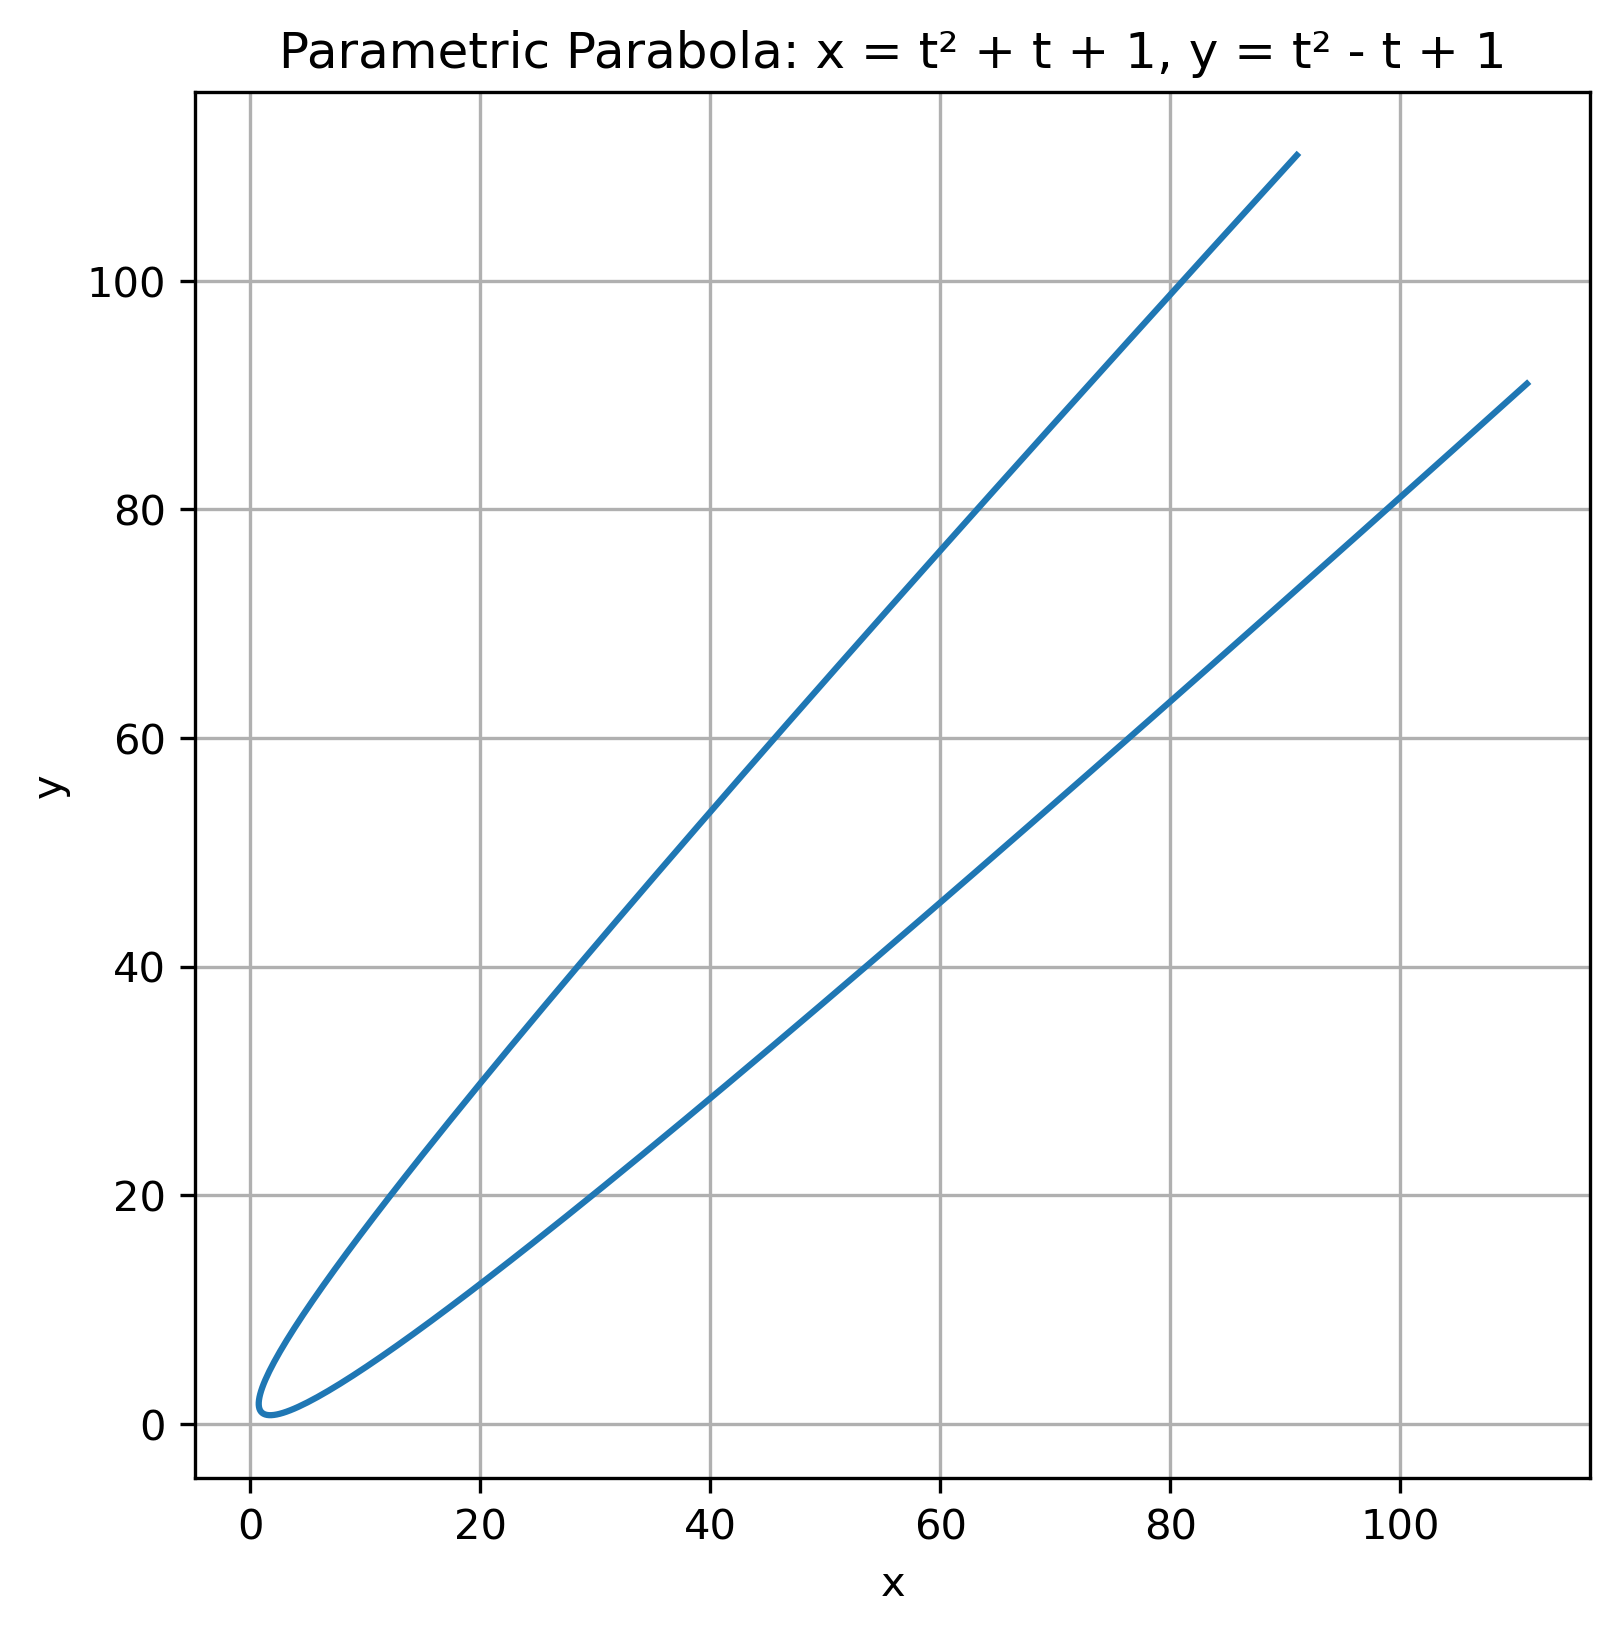
\includegraphics[scale=0.5]{img1}
	\caption*{}
	\label{img1}
\end{figure}
Plot using Python:
\begin{figure}[H]
	\centering
	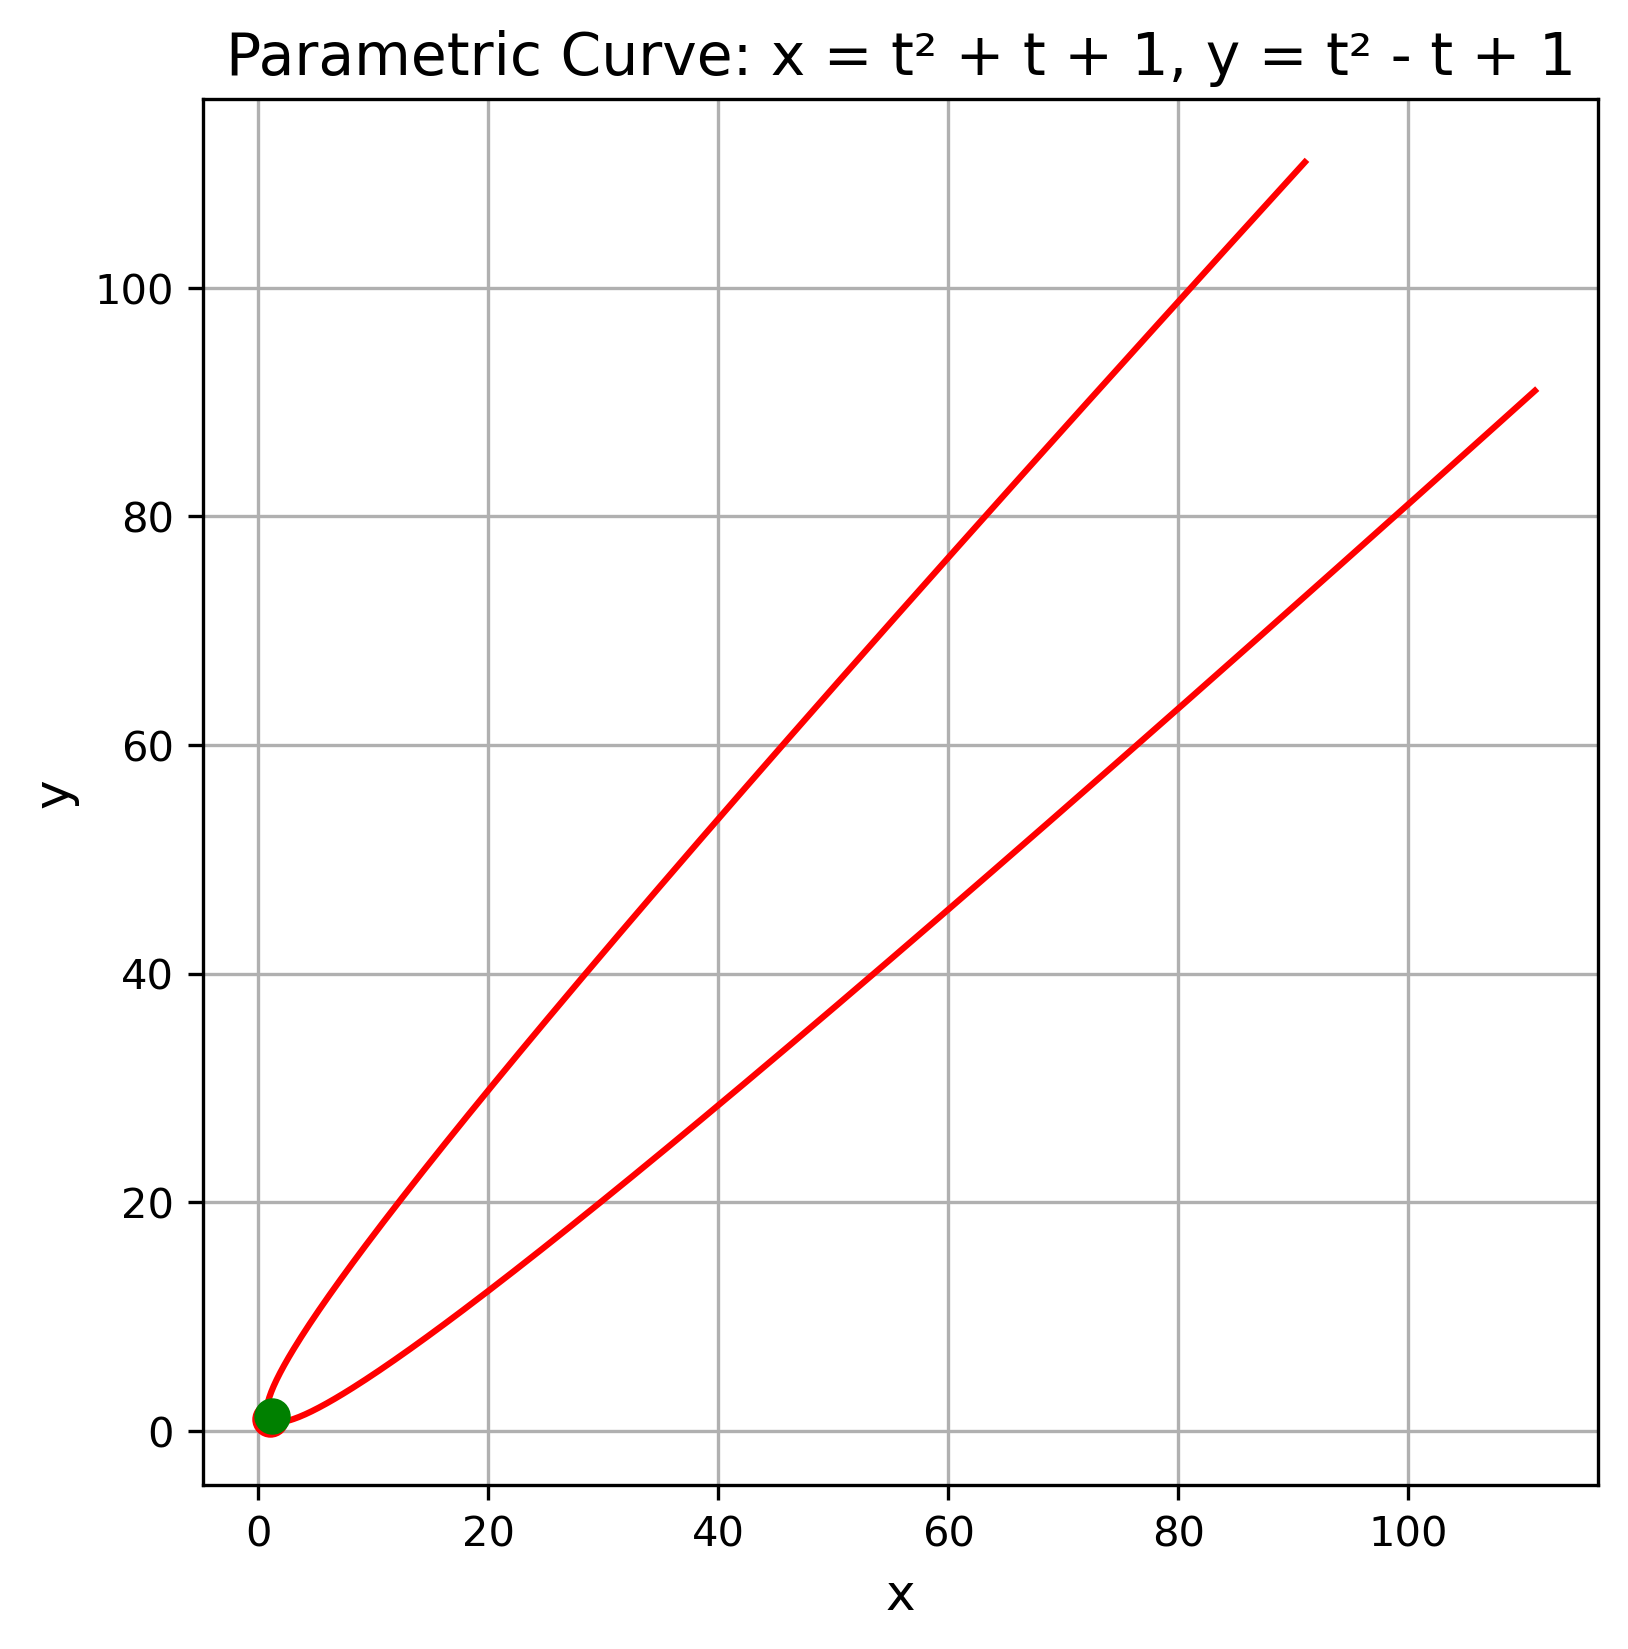
\includegraphics[scale=0.5]{img2}
	\caption*{}
	\label{img2}
\end{figure}

\end{document}
